\label{sec:3}

\section{Repository Overview}
\label{sec:3.1}

\begin{table}[htb]
\centering
\renewcommand{\arraystretch}{1.2}
\begin{tabular}{l@{\hspace{1cm}}p{0.55\textwidth}}
\textbf{Path} & \textbf{Description} \\
\midrule
\texttt{src/main.py} & Entry point for individual simulation runs. \\
\texttt{src/tune.py} & Entry point for parameter-tuning simulation runs. \\
\texttt{src/validate.py} & Entry point for behavioural and kinematic validation simulation runs. \\
\midrule
\texttt{src/simulation/simulation.py} & Simulation kinematics and lifecycle manager. \\
\texttt{src/simulation/mdp.py} & MDP framework, \texttt{FastMDP} implementation and reward functions. \\
\midrule
\texttt{src/outputs/base.py} & Output manager and base output type component. \\
\texttt{src/outputs/*.py} & Output type implementations (e.g. plot, video). \\
\texttt{src/display.py} & Terminal dashboard set-up and lifecycle. \\
\texttt{src/visualisation.py} & \texttt{pyvista} interactive 3D visualisation. \\
\texttt{results/} & Directory for any produced outputs. \\
\midrule
\texttt{src/assets/} & Public-use models for use in 3D visualisation. \\
\texttt{src/configs/} & Configuration values for project components. \\
\texttt{tests/} & Unit tests for project components. \\
\end{tabular}
\caption{Repository structure}
\label{tab:repo}
\end{table}

The simulation and machine learning functionality were coded from scratch without reliance on pre-existing code or external libraries. A selection of features from the Python standard library and mainstream libraries were used:
\begin{itemize}[nosep]
    \item \texttt{rich} for clear and colourful terminal logs and interfaces.
    \item \texttt{pytest} for unit test management.
    \item \texttt{numpy} for efficient N-dimensional numerical computation.
    \item \texttt{matplotlib} and \texttt{asciichartpy} for standard data plotting functionality.
    \item \texttt{pyvistaqt} and \texttt{pyqt5} for the interactive 3D visualisation.
    \item \texttt{numba} for JIT compilation of computationally-heavy Python code to machine code at runtime (described further in Extensions).
\end{itemize}
In all cases, the relevant library provided generic functionality that assisted with performance or visualisation, and additional code was written to interoperate with the simulation implementation.

Before beginning development, the project scaffolding was set up. A \texttt{pytest} configuration was set up with a dedicated test folder importing source components, and a GitHub Actions workflow was configured to run the full test suite automatically on every push to the remote repository. The \texttt{argparse} standard library was used in a \texttt{main.py} file to provide a base command-line interface for configuring and launching simulation runs. The project supported configuration of many key values. Unless otherwise stated, all examples and evaluation in this dissertation use the base configuration included in Appendix C.

\Cref{fig:system} gives an architectural overview of the final system, explored in detail throughout this chapter.

\begin{figure}[htb]
\centering
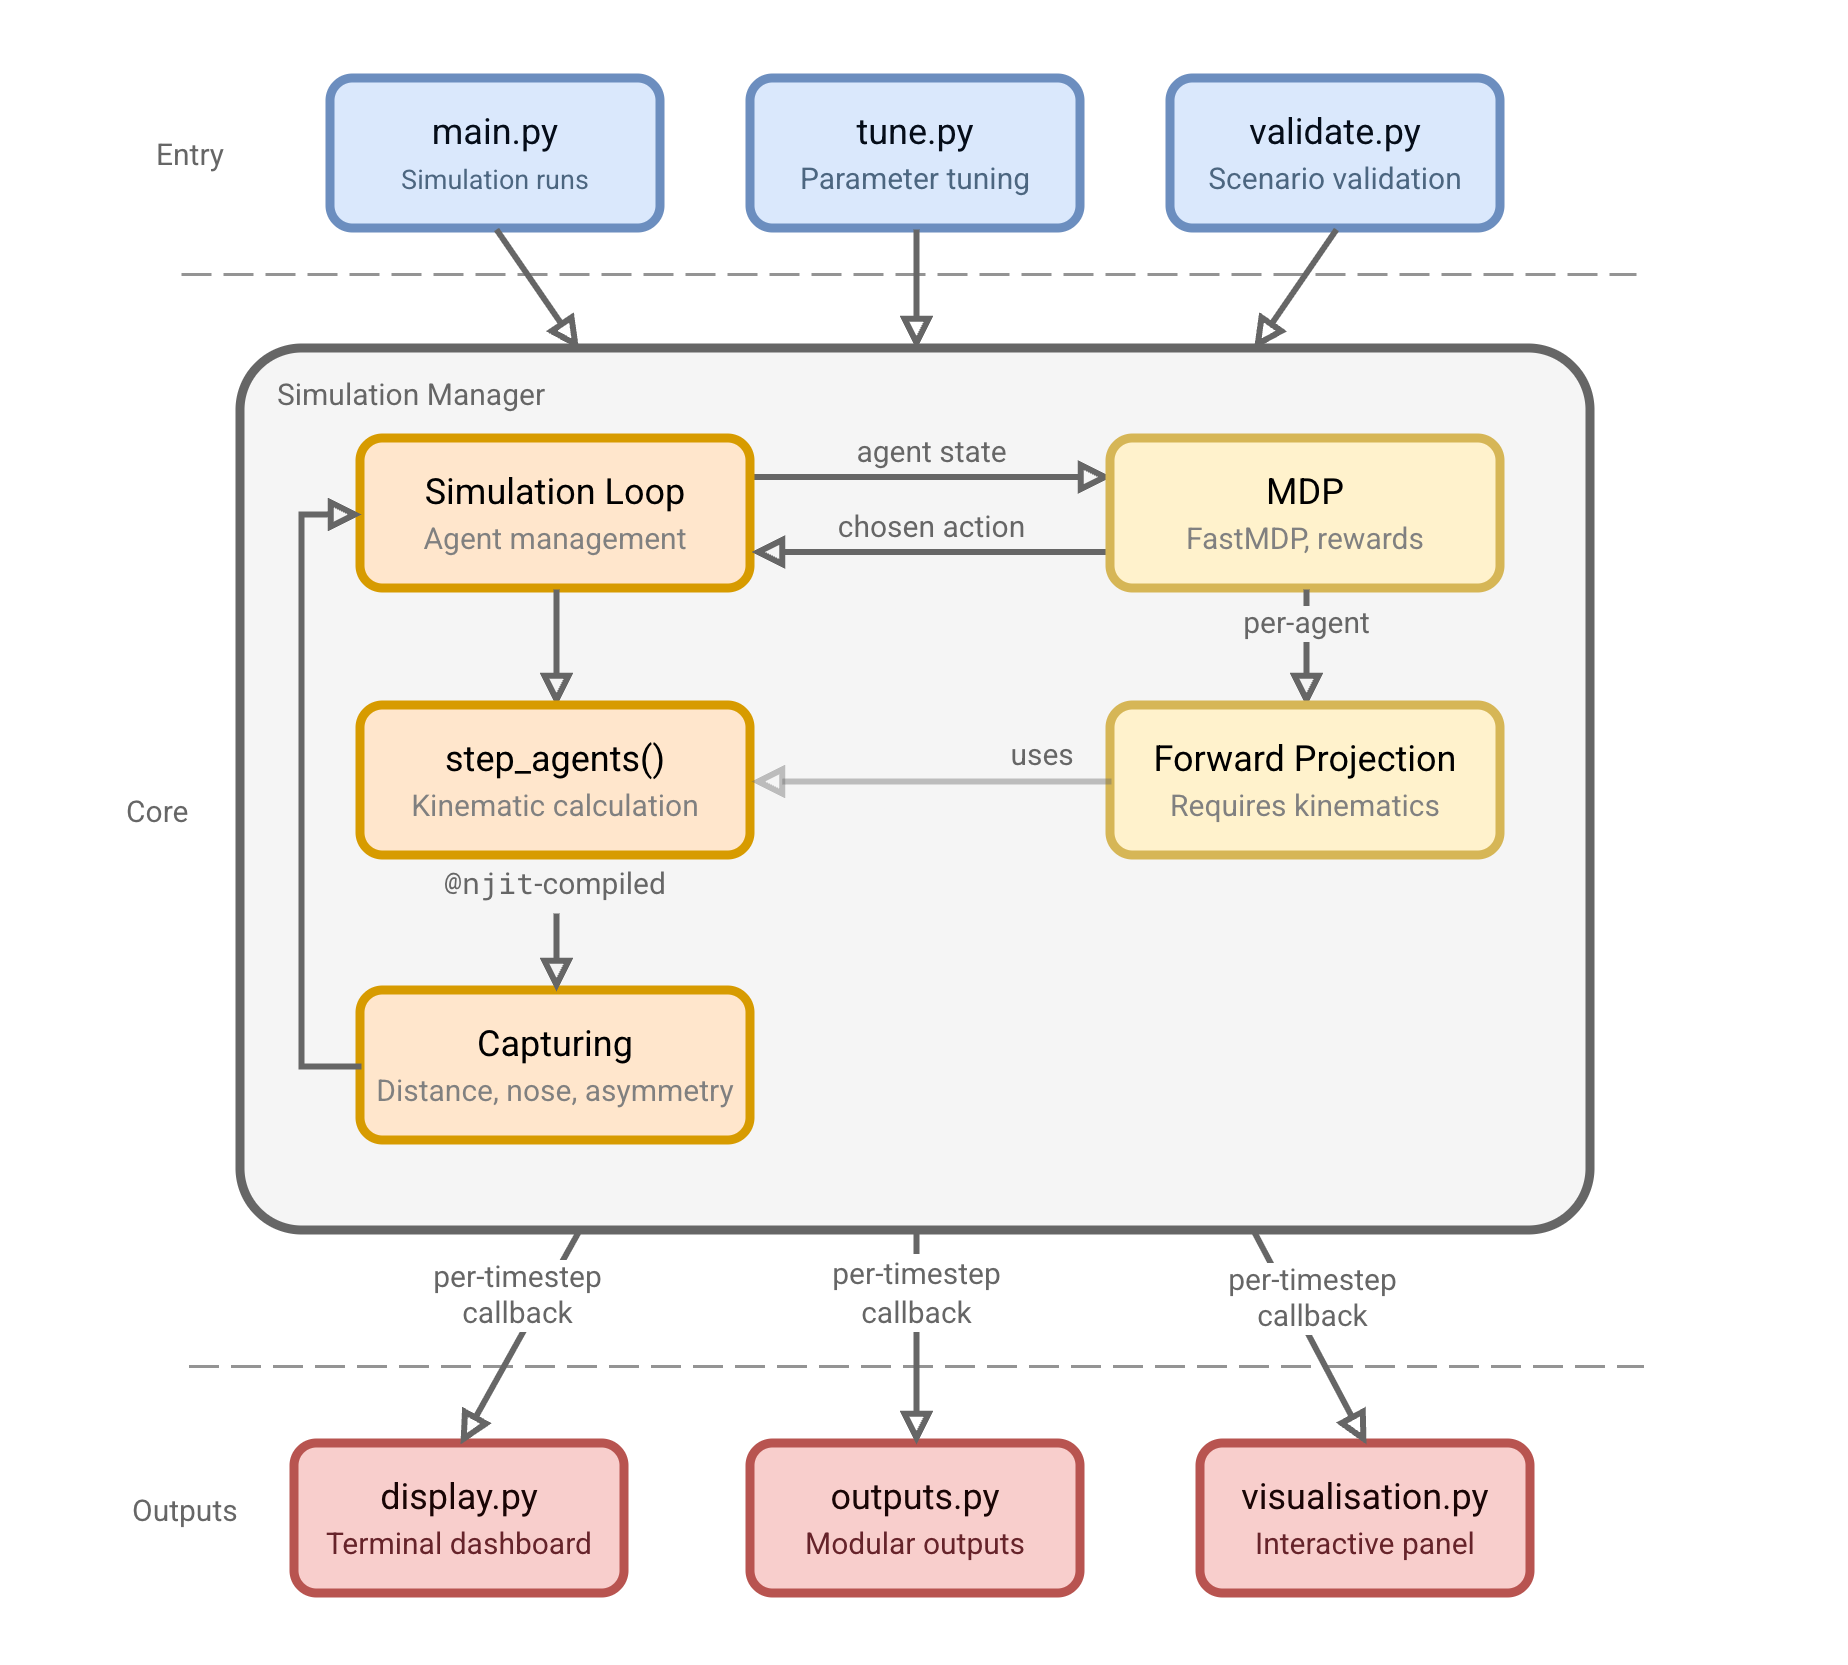
\includegraphics[width=\textwidth]{figures/system.png}
\caption{System architecture}
\label{fig:system}
\end{figure}

\section{Kinematic Model}
\label{sec:3.2}
The kinematic model was developed in incremental steps up to three-dimensionality with pursuit-evasion behaviour expanded at each stage. This allowed for smoother integration of other components (outputs, visualisations), and for the decision-making functionality to be examined and debugged in much simpler environments before presenting a full solution. The target was a full three-dimensional pseudo-6DoF model as described in the Preparation chapter.

In all cases, time was discretised with a \texttt{STEPS\_PER\_SECOND} configuration value to give a timestep variable $dt = 1 / \texttt{STEPS\_PER\_SECOND}$ for kinematic calculations. Each kinematic value can be updated as $x_{t+1} = x_t + \dot{x} \cdot dt$ through 
semi-implicit Euler integration for multiple equations, following the discrete-time approach of Bertram et al.\cite{bertram3d}.

\subsection{One- and Two-Dimensionality}
\label{sec:3.2.1}
The aim of one-dimensional kinematics was primarily to validate the simulation timestepping framework and agent system. The space is defined with a right-positive convention and agents are represented with a position and a velocity. The action space is a set of discrete acceleration (m/s$^2$) values $\{a_1, a_2, \dots, a_n\}$ with velocity (m/s) updated as $v_{t+1} = v_t + a_{\text{chosen}} \cdot dt$ and position (m) as $p_{t+1} = p_t + v_{t+1} \cdot dt$, all in base SI units. The system interfaced with a naive version of the \textit{FastMDP} algorithm described in \cref{sec:3.3} and a simple output system, and the resulting trajectories shown in \cref{fig:1d_plot} confirmed that a decision-making agent approaches its opponent.

\begin{figure}[htb]
    \centering
    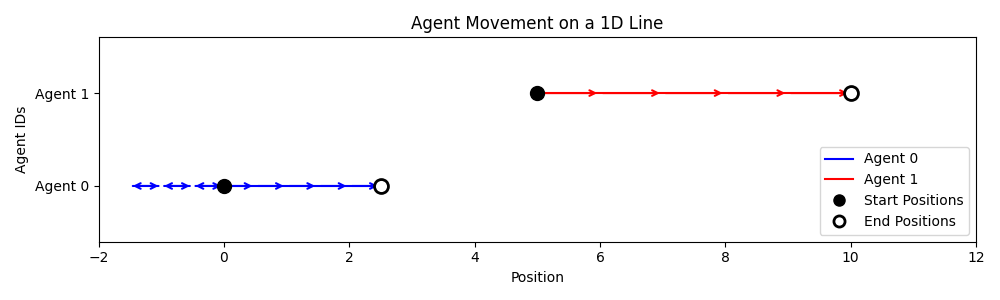
\includegraphics[width=\textwidth]{figures/visualisation/1d_plot.png}
    \caption{1D Simulation Plot}
    \label{fig:1d_plot}
\end{figure}

\review{do i need to do anymore work on this plot? its just here in its raw state as a development aid, and its effectivness as an visualiastion is considered in Evaluation (spoiler alert: its not great)}

The codebase was initially object-oriented as determined in my design preparation. A \texttt{Simulation} singleton maintained a list of \texttt{Agent} objects that encapsulated their own kinematic state. This was a natural design given the conceptual clarity of individual agent entities. The decision-making framework also supported this design, as per-agent MDPs could be instantiated from a single class with relevant parameters. A \texttt{step()} method could be run each timestep to determine actions, apply them and update kinematic values for each agent. 

It became apparent in early development that this design was incompatible with eventual intended optimisations. Individual agent object updates could not take advantage of NumPy's array broadcasting, and Numba's JIT compilation incurred a significant performance penalty when interfacing with arbitrary objects rather than raw procedures.

The aim of two-dimensional kinematics was to more deeply explore the \textit{FastMDP} algorithm and possible reward functions. This would require a base level of optimisation, so I decided to refactor the codebase design to address the above issues. Kinematic calculations were extracted to a single \texttt{step\_agents()} method that accepted flat arrays of agent state and applied updates across all $N$ agents simultaneously using NumPy's vectorised operations. This was also a clean interface for later investigating Numba's no-Python JIT compilation mode (described in \cref{sec:3.5.1}).

Two-dimensional kinematics introduced a heading parameter $\psi$ measured in radians, replaced acceleration with thrust value $n_x$ and expanded position and velocity to 2-vectors. The action space became $\{(\dot{\psi},n_x)\}$, and the numerical integration is shown in \cref{lst:step_agents_2d}.

\begin{listing}[H]
\begin{minted}{python}
# input values: heading_rates, thrusts (applied across N agents)
headings = headings + heading_rates * dt

ax = thrusts * np.cos(headings)
ay = thrusts * np.sin(headings)
accelerations = np.stack((ax, ay), axis=-1)

velocities = velocities + accelerations * dt
positions = positions + velocities * dt

return (positions, velocities, headings)
\end{minted}
\caption{2D kinematic updates via semi-implicit Euler integration using vectorised operations.}
\label{lst:step_agents_2d}
\end{listing}

The 2D exploration of pursuit-evasion behaviour is described in \cref{sec:3.3}.

\todo{video artefact of 2d pursuit evasion to include?}

\subsection{Three-Dimensionality}
\label{sec:3.2.3}

Three-dimensional kinematics were introduced midway through the project, after a modular output system and the majority of the MDP framework had been implemented, and significantly expanded on the 2D implementation. The agent state grew to include speed $V$, attack angle $\alpha$, flight path angle $\gamma$, roll angle $\phi$, and azimuth angle $\psi$ in addition to position, following the pseudo-6DoF model described in the Preparation chapter. The action space became $\{(n_x, \dot{\alpha}, \dot{\phi})\}$ with thrust $n_x$, attack angle rate $\dot{\alpha}$ and roll angle rate $\dot{\phi}$ as inputs. The normal force $n_f$ is derived as a speed-dependent G-load.

The equations of motion from Bertram and Wei\cite{bertram3d} are implemented directly:

\begin{listing}[H]
\begin{minted}{python}
max_g_at_speed = np.minimum(MAX_GS, MAX_GS * (velocities / CORNER_VELOCITY) ** 2)
nf = alpha * max_g_at_speed
turn_drag = K_DRAG * (nf ** 2)

speed_rates = 
    g * 
    (thrusts - turn_drag - np.sin(flight_path_angles))

flight_path_angles_rates = 
    (g / speeds) * 
    (nf * np.cos(roll_angles) - np.cos(flight_path_angles))

azimuth_angles_rates = 
    (g * nf * np.sin(roll_angles)) / 
    (speeds * np.cos(flight_path_angles))
\end{minted}
\caption{3D kinematic rate calculations following the designed pseudo-6DoF model.}
\label{lst:kinematic_rates}
\end{listing}

Realistic kinematic bounds are enforced through value clipping after integration, with configurable minimums and maximums per-agent to compare parameters.

\begin{table}[H]
\centering
\renewcommand{\arraystretch}{1.2}
\begin{tabular}{l@{\hspace{1cm}}l@{\hspace{1cm}}l}
\textbf{Parameter} & \textbf{Range} & \textbf{Units} \\
\midrule
Speed $V$ & $[34.3, 103.0]$ & m/s (0.1--0.3 Mach) \\
Azimuth rate $\dot{\psi}$ & $[-1.3, 1.3]$ & rad/s \\
Attack angle $\alpha$ & $[0.09, 0.52]$ & rad (5°--30°) \\
Flight path angle $\gamma$ & $(-\pi/2, \pi/2)$ & rad \\
Hard deck & $z > 0$ & m \\
Arena & $10{,}000 \times 10{,}000 \times 10{,}000$ & m \\
\end{tabular}
\caption{Base kinematic bounds and arena configuration.}
\label{tab:kinematic_bounds}
\end{table}

The speed and angular state are resolved to a velocity vector for the position update:

\begin{listing}[H]
\begin{minted}{python}
vx = speeds * np.cos(flight_path_angles) * np.cos(azimuth_angles)
vy = speeds * np.cos(flight_path_angles) * np.sin(azimuth_angles)
vz = speeds * np.sin(flight_path_angles)
velocities = np.stack((vx, vy, vz), axis=-1)
positions = positions + velocities * dt
\end{minted}
\caption{Scalar speed and angles resolved to a 3D velocity vector for position update.}
\label{lst:velocity_resolution}
\end{listing}

The \texttt{step\_agents()} function is fully compatible with the \texttt{@njit} decorator for Numba's no-Python mode.

The progression from 1D to 3D affected my software methodology throughout implementation. In some cases, heavy refactoring of the codebase design (such as the move away from OOP) clashed with the agile approach - instead of iterating on previous work and integrating features, structural core changes required additional design work and re-interfacing with existing components. I was still able to adapt to the changing requirements and the incremental progressions had clear functional goals to work towards.
Refactoring also impacted the test suite. Tests that had been written against earlier interfaces were invalidated and coverage reduced. The CI pipeline identified these issues and maintaining the tests was not an issue, but this was a limitation of the testing approach that I could evaluate later. 

\review{three dimensional output? video? plot? visualisation screenshot? should that wait until the reward function/decision behaviour is described?}

\subsection{Capturing}
\label{sec:3.2.4}

The capturing mechanic tied into the kinematic system. A simulation ends after a maximum number of timesteps, or when all but one agent has been captured. The capturing condition laid out during preparation involved being within a configurable distance of a control point 3 seconds behind an enemy, and aligned towards them within some limit. I found this did not result in accurate-looking capture during examination of the visualisation, so redesigned the criteria during development.

The following must hold simultaneously true for $N$ consecutive timesteps for a capture to occur:

\begin{enumerate}[nosep]
    \item \textbf{Distance check}: the Euclidean distance between agents falls within a capture radius $r$.
    \item \textbf{Nose check}: the pursuer's nose direction is within 50\textdegree~of the evader.
    \item \textbf{Asymmetry check}: the pursuer has a meaningfully better alignment than the evader, $a_\text{pursuer} > a_\text{evader} + 0.2$.
\end{enumerate}

These conditions were designed from scratch and are an original contribution to the problem space investigated in the project. Fragments of implementation can be seen in \cref{lst:captures}. These conditions also guided the eventual design of the reward functions in \cref{sec:3.3.3}.

\begin{listing}[H]
\begin{minted}{python}
r_pe = evader_position - pursuer_position
d = np.linalg.norm(r_pe)
r_pe_hat, r_ep_hat = r_pe / d, -r_pe / d

pursuer_alignment = np.dot(pursuer_nose, r_pe_hat)
evader_alignment = np.dot(evader_nose, r_ep_hat)

distance_check = d < SimulationConfig.CAPTURE_RADIUS
nose_check = pursuer_alignment >= np.cos(np.deg2rad(50))
asymmetry_check = pursuer_alignment > evader_alignment + 0.2
\end{minted}
\caption{Capture condition values and comparisons}
\label{lst:captures}
\end{listing}

With three-dimensional kinematics and capturing implemented, the core simulation loop was finalised (\cref{lst:sim_loop}). The simulation steps all agents forward by determining their next action and applying kinematic updates. Captures are calculated and applied, out-of-module callbacks are triggered, and ending conditions are checked.

\begin{listing}[H]
\begin{minted}{python}
while self.simulation.timestep < SimulationConfig.MAX_TIMESTEPS:
    self.simulation.step()
    captures = self.simulation.determine_captures()

    for captured_id, capturer_id in captures:
        all_captures.append(
            (self.simulation.timestep, captured_id, capturer_id)
        )

    for callback in callbacks:
        callback(self.simulation)

    if np.sum(self.simulation.active) <= 1:
        break
\end{minted}
\caption{Simulation loop with capture-breaking logic and per-timestep callbacks}
\label{lst:sim_loop}
\end{listing}

\section{Decision Making}
\label{sec:3.3}
The decision-making framework is clearly separate from the simulation component, and implements the \texttt{FastMDP} algorithm with novel reward functions refined through a parameter tuning process.

\subsection{\texttt{FastMDP}}
\label{sec:3.3.1}

The full \texttt{FastMDP} algorithm was initially implemented alongside two-dimensional kinematics to examine behaviour in a simpler environment. This component remained object-oriented - an \texttt{MDP} class is constructed per-agent per-timestep exposing the following methods:

\begin{itemize}[nosep]
    \item \texttt{find\_action} to run the reward-action maximising loop.
    \item \texttt{calculate\_rewards} to combine positive and negative rewards into a single surface.
    \item Two reward functions to compute the positive and negative value functions. 
    \item \texttt{hard\_deck\_penalty} to add a very high negative penalty separate to the parameterised negative rewards when an agent approaches $z = 0$.
\end{itemize}

At each timestep, before any agent's MDP is solved, all agents are forward projected using zero actions to produce a central world state. Each agent then uses this world state as reward sources - the positions and velocities other agents will reach if they continue on their current trajectory — rather than their current positions. This provides a more accurate reward signal.

\Cref{lst:find_action} shows the implementation of the core decision-making loop. In practice, \texttt{current\_state} represents the full set of kinematic arrays that are passed individually into the MDP and forward projection process for Numba compatibility, but is simplified here for clarity.

\begin{listing}[H]
\begin{minted}{python}
def find_action(self, current_state) -> Action:
    from simulation import forward_project

    num_actions = self.actions.shape[0]
    action_rewards = np.zeros(num_actions)

    # Choose each action
    for i in range(num_actions):
        action = actions[i]

        # Project self agent forward with that action
        projected_positions, projected_velocities = 
            forward_project(FORWARD_PROJECTION_STEPS, current_state, *action)

        # Calculate reward from resulting values
        action_rewards[i] = self.calculate_reward(
            projected_positions, 
            projected_velocities
        )

    # Choose best action
    best_action = actions[np.argmax(action_rewards)]
    return best_action

\end{minted}
\caption{\texttt{FastMDP} action selection via forward projection and reward evaluation.}
\label{lst:find_action}
\end{listing}

\Cref{lst:forward_project} demonstrates how forward projection was straightforward to implement using the standalone \texttt{step\_agents} function from the simulation module. The Numba-provided \texttt{prange} function allowed \texttt{forward\_project} to be JIT compiled in the same manner.  

\begin{listing}[H]
\begin{minted}{python}
@njit
def forward_project(steps, current_state, thrust, azimuth_angle_rate, roll_angle_rate):
    for _ in prange(steps):
        current_state = step_agents(current_state, thrust, attack_angle_rate, roll_angle_rate)
    return current_state
\end{minted}
\caption{Forward projection applies an action to a specific agent for a fixed number of steps.}
\label{lst:forward_project}
\end{listing}

In two-dimensional kinematics, the action space was a finite set of heading turn rates and acceleration values. The reward functions were only position-based and placed positive rewards at enemy positions to drive pursuit.

When I expanded the simulation to 3D kinematics the state and inputs became more complex. The action space constructed as the Cartesian product of configurable ranges of the three kinematic inputs described in the Preparation chapter: thrust, attack angle rate and roll angle rate. These are scaled by ratio values to support heterogeneous agent configurations:

\begin{listing}[H]
\begin{minted}{python}
self.actions = np.array(
    [
        [
            thrust * thrust_ratio,
            attack_angle * attack_angle_ratio,
            roll_angle * roll_angle_ratio,
        ]
        for thrust in MDPConfig.ACTION_THRUSTS
        for attack_angle in MDPConfig.ACTION_ATTACK_ANGLE_RATES
        for roll_angle in MDPConfig.ACTION_ROLL_ANGLE_RATES
    ]
)
\end{minted}
\caption{Action space generation from configurable ratios.}
\label{lst:action_space}
\end{listing}

\subsection{Parameter Analysis}
\label{sec:3.3.2}
To inform the design of the final reward functions, a One-at-a-Time sensitivity analysis was performed on the system. A tuning process evaluated the effect of increasing kinematic bound ratios between agents in a 1v1 arena. Starting from an equal base configuration, the script generated linear spaces for each parameter and ran a full simulation until capture or max timestep. 

The results of these simulations were visualised in two ways. \Cref{fig:parameter_panels}
shows a grid of timesteps to capture against parameter value for each investigated parameter individually. \Cref{fig:paramter_compare} maps all parameter ranges onto a normalised scale and plots the percentage change in timesteps to capture from the baseline. This allowed a direct comparison of gradients and helped evaluate the dominant parameters.

\begin{figure}[H]
\centering
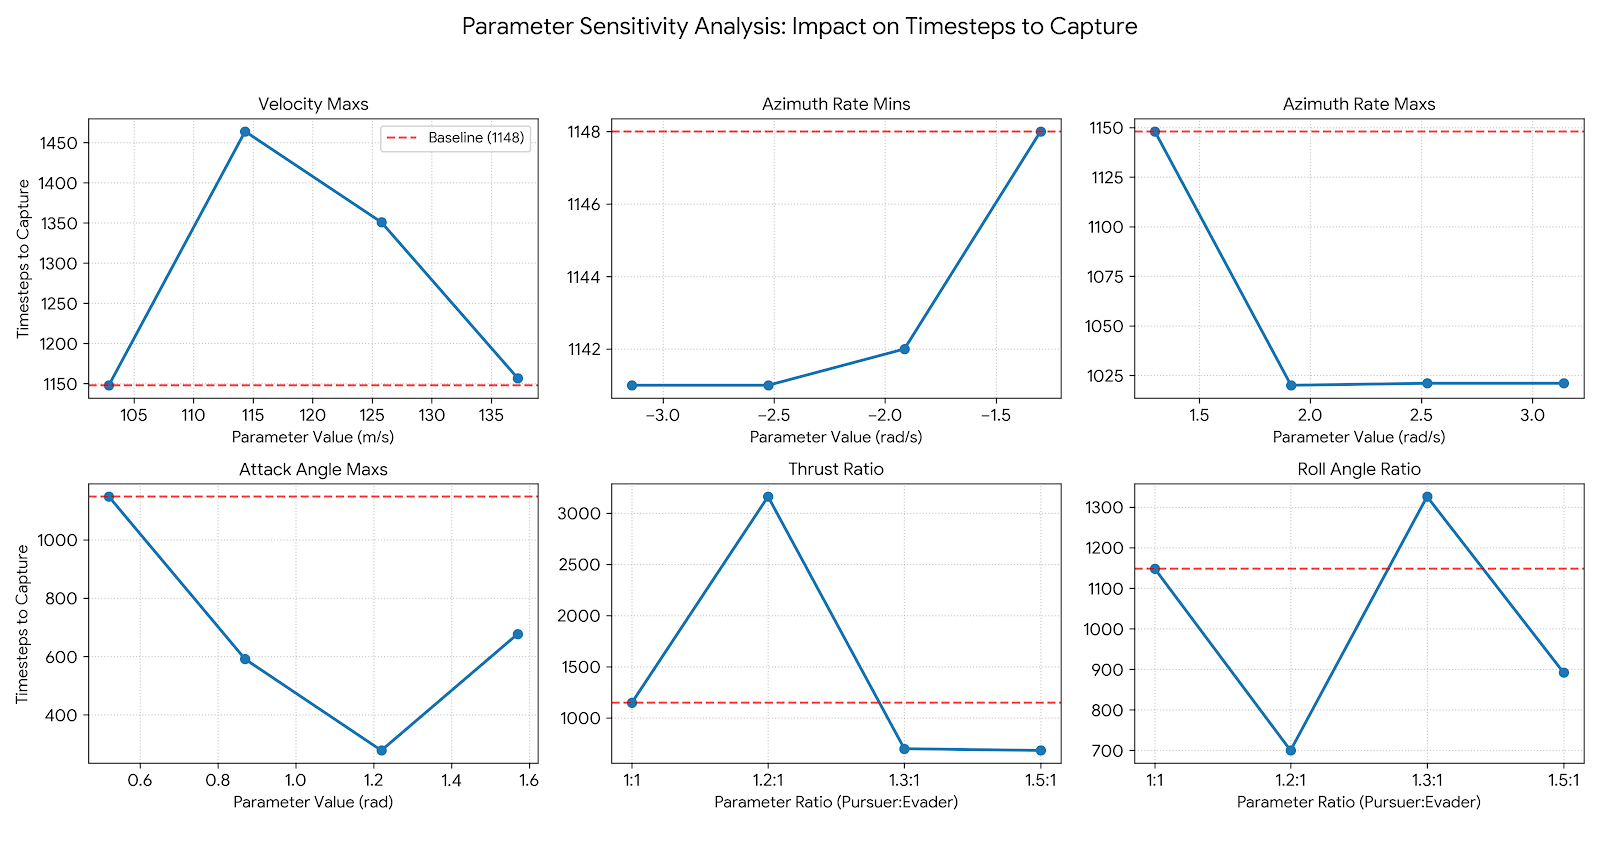
\includegraphics[width=\textwidth]{figures/parameters_separate.png}
\caption{One-at-a-Time sensitivity analysis: timesteps to capture against parameter value.}
\label{fig:parameter_panels}
\end{figure}

\begin{figure}[H]
\centering
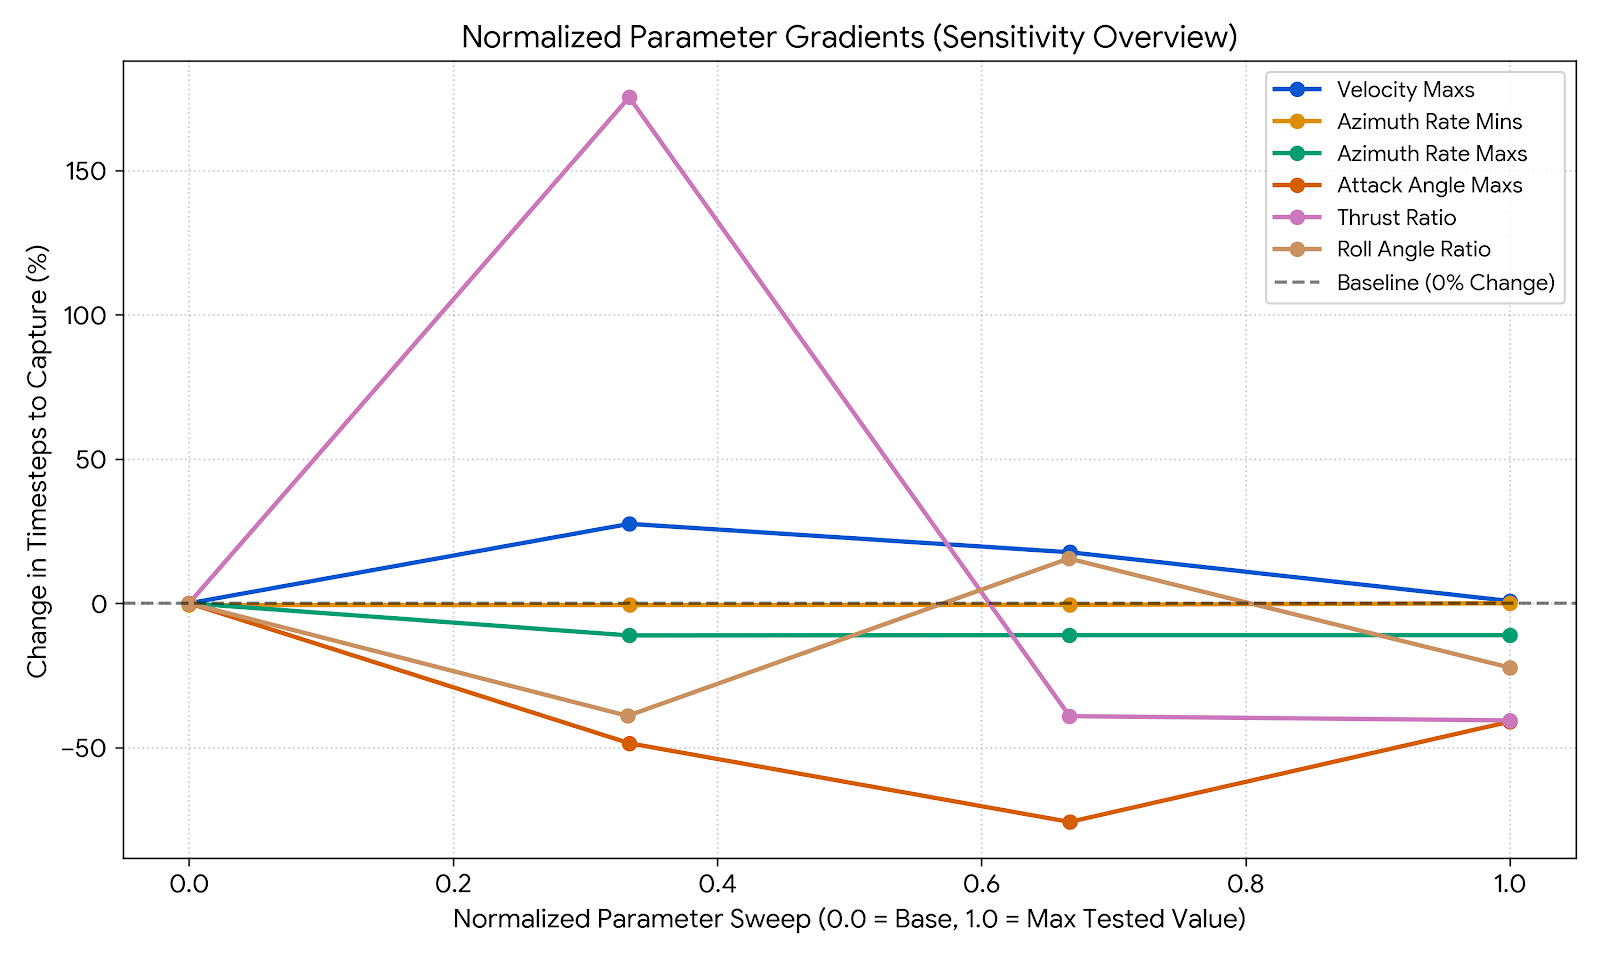
\includegraphics[width=\textwidth]{figures/parameter_together.png}
\caption{Normalised gradients showing percentage change in timesteps to capture from baseline for each parameter investigated.}
\label{fig:paramter_compare}
\end{figure}

Attack angle maximum was the dominant parameter, reducing timesteps to capture by approximately 75\% at its optimal value --- a larger effect than any other parameter. Azimuth rate maximum showed a consistent improvement, confirming that turning capability is a meaningful pursuit advantage. Thrust ratio and velocity maximum showed non-monotonic behaviour, initially increasing timesteps to capture before improving beyond the baseline, which suggested an optimal operating range. Azimuth rate minimum and roll angle ratio had comparatively small effects overall.

These results further motivated the design of alignment-based reward instead of positioning-based ones, as the angular maximum parameters had the greatest effect on pursuit efficiency.

\subsection{Reward Functions}
\label{sec:3.3.3}

After investigating the effects of kinematic parameter and bound ratios, reward functions were designed that considered alignment properties when creating the value function surface for the MDP. 

\begin{listing}[H]
\begin{minted}{python}
def positive_maximum(
    self_position: Vector,
    self_velocity: Vector,
    other_positions: Vectors,
    other_velocities: Vectors,
) -> float:
    r = other_positions - self_position
    d = np.linalg.norm(r, axis=1)
    r_hat = r / d[:, np.newaxis]

    # Self pointing toward enemy
    self_v_hat = self_velocity / np.linalg.norm(self_velocity)
    pursuit_alignment = np.dot(r_hat, self_v_hat)

    # We are in enemy's rear hemisphere
    enemy_v_hat = (
        other_velocities / np.linalg.norm(other_velocities, axis=1)[:, np.newaxis]
    )
    r_from_enemy = -r_hat  # vector from enemy to self
    aspect_alignment = -np.sum(r_from_enemy * enemy_v_hat, axis=1)

    score = (pursuit_alignment + aspect_alignment) / d

    return np.max(score)
\end{minted}
\caption{Positive reward function.}
\label{lst:positive}
\end{listing}

Angular limits had a large effect on pursuit efficiency, so the positive reward function in \cref{lst:positive} evaluates relative geometry between the agent and opponents. The first term, \texttt{pursuit\_alignment}, measures alignment between the agent's velocity and the line-of-sight to each opponent to encourage motion towards the target. The second term, \texttt{aspect\_alignment}, measures the inverse alignment from the opponent and favours being in their rear hemisphere to avoid capture.
These terms are summed and inversely scaled by distance to result in the maximal positive reward for close, well-aligned configurations.

\begin{listing}[H]
\begin{minted}{python}
def negative_maximum(
    self_position: np.ndarray,
    other_positions: np.ndarray,
    other_velocities: np.ndarray,
) -> float:
    r = other_positions - self_position
    d = np.linalg.norm(r, axis=1)
    r_hat = r / d[:, np.newaxis]

    enemy_v_hat = (
        other_velocities / np.linalg.norm(other_velocities, axis=1)[:, np.newaxis]
    )

    # Calculate alignment
    alignment = np.sum(-r_hat * enemy_v_hat, axis=1)

    # Only penalise if the enemy alignment > 0 (pointing towards self)
    threat_score = np.maximum(0, alignment) / d

    return np.max(threat_score)
\end{minted}
\caption{Negative reward function.}
\label{lst:negative}
\end{listing}

The negative reward function in \cref{lst:negative} measures the threat from each opponent by considering their orientation towards the agent. This value is also scaled by distance, and clamped to $0$ for opponents not actively threatening the agent. The two rewards provide pursuit behaviour through velocity alignment towards a target, whilst simultaneously evading being in a target's line-of-sight. A very large ($1 \times 10^9$) negative reward is separately applied for any agents below the hard deck of $z = 0$.

\begin{listing}[H]
\begin{minted}{python}
best_positive_reward = positive_maximum(*self_state, *others_state)
best_negative_reward = negative_maximum(*self_state, *others_state)
total_reward = best_positive_reward - best_negative_reward
total_reward -= self.hard_deck_penalty(self_position)

return total_reward
\end{minted}
\caption{Calculate final reward.}
\label{lst:combine}
\end{listing}

\review{is the above listing necessary? could just descirbe in prose how they are summed and hard deck penalty applied}

\review{possibly place the 3D visualisation video here?}

\section{Output System}
\label{sec:3.4}

Being able to visualise simulation runs in various ways was a key requirement during development. Qualitative analysis of flight paths, trajectories and agent interactions helped debug kinematic issues and shape the reward functions.

\subsection{Plots and Videos}
\label{sec:3.4.1}
There was a requirement to fully represent the results of a simulation run to inform development and evaluation. Static plots of agent trajectories provided a limited overview, but video outputs allowed them to be observed over time. A modular output manager was implemented that registered a callback with the simulation manager to save agent state each timestep. An abstract \texttt{Output} class could be implemented to access this data and save it into various formats. 

The \texttt{PlotOutput} and \texttt{VideoOutput} concrete classes were written to produce simulation visualisations. They worked well, especially for two-dimensional kinematics. 

\begin{listing}[H]
\begin{minted}{python}
for agent_idx, agent_path in enumerate(self.output_manager.agent_paths):
    # Extract positions and stack into (N,3) array
    positions = np.stack([pos for pos, _, _, _, _ in agent_path])

    if len(positions) > 1:
        # Plot the path
        self.ax.plot(
            *positions.T,
            label=f"Agent {agent_idx}",
            linewidth=1.5,
            linestyle=linestyles[agent_idx % len(linestyles)],
        )
\end{minted}
\caption{Plot agent paths on a \texttt{matplotlib} 3D graph, discarding unused kinematic data.}
\label{lst:plot}
\end{listing}

\review{add video artefact? point again to one that was used earlier?}

There were two key limitations to this approach. First, outputs were only produced after a simulation run completed, so there was no way to inspect agent behaviour mid-run. Second, while one- or two-dimensional trajectories could be represented clearly, three-dimensional environments were limited by fixed perspective or camera paths.

\subsection{Terminal Dashboard}
\label{sec:3.4.2}
A terminal dashboard was created after implementing the core simulation framework and two-dimensional kinematics to address these issues. It was created with the \texttt{rich} library and provided a real-time representation of simulation state. There were two core panels - a display of key values from the simulation at each timestep, and a top-down orthographic projection of agent positions. Additionally there were graphs of CPU usage and memory usage to monitor system metrics throughout the simulation, but these were not fully accurate and were eventually removed in favour of separate performance trackers. 

The dashboard (a version of which with the system metrics can be seen in \cref{fig:dashboard}) was designed to aid rapid iteration and development. Staying in the development terminal allowed me to run a simulation and immediately sanity check values - e.g initial agent positions and headings or parameter ratios, and its clear layout aided with obvious interpretation. It was primarily a development tool but a good time investment and remained in use until the end of the project.

\begin{figure}[htb]
\centering
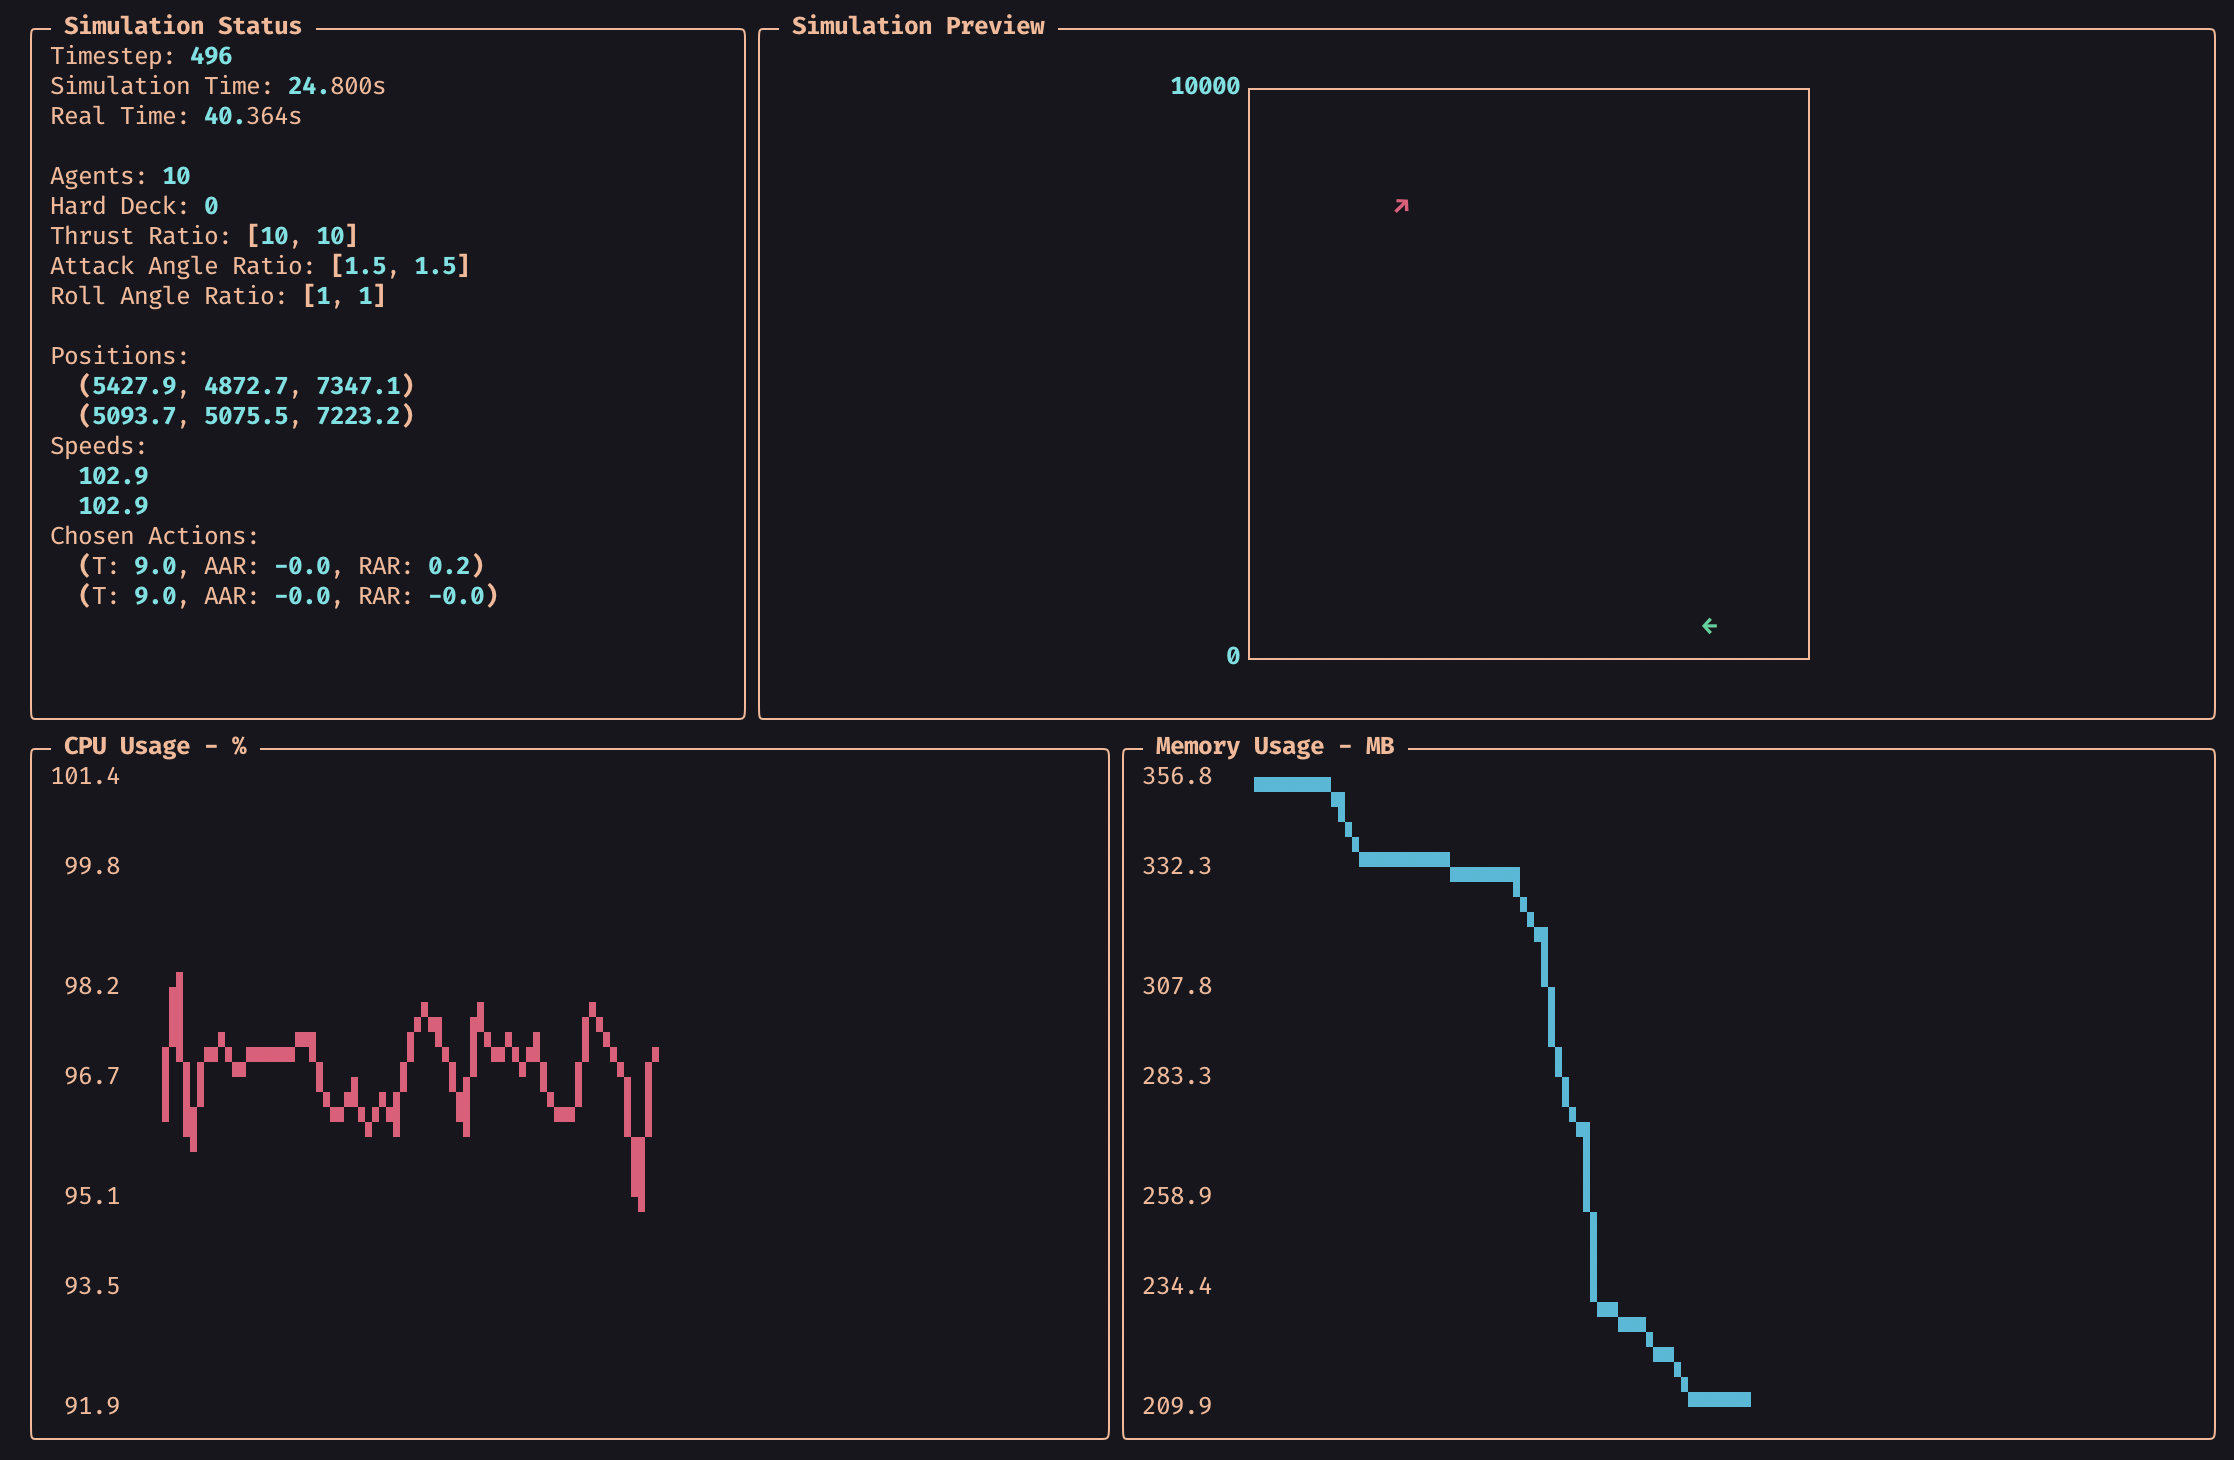
\includegraphics[width=\textwidth]{figures/terminal_dashboard.png}
\caption{Terminal Dashboard}
\label{fig:dashboard}
\end{figure}

\subsection{Interactive Visualisation}
\label{sec:3.4.3}

The final milestone in the output system was a 3D visualisation of the current simulation run implemented with the \texttt{pyvista} library, chosen for its interactivity support. It exists inside a \texttt{Qt} GUI window which allows for interactive panning, zooming and rotating throughout the simulation run. The application window runs alongside the simulation on a separate thread, registering a callback to update visualised agents (rendered with public-use aircraft models) at each timestep. At close camera ranges, additional velocity direction indicators and speed labels appear by each agent, providing more granular state detail on demand as seen in \cref{fig:3d_visuals}. Users can freely rotate their perspective to examine the simulation and agent behaviour. 

\texttt{pyvista} provided the base platform and interaction functionality, but interoperating code had to be written to add actor meshes to the scene, trigger position updates and manage the rendering loop. A key step involved transforming kinematic angles from the simulation space to the world space of the visualisation, as seen in \cref{lst:pyvista}.

\begin{listing}[H]
\begin{minted}{python}
def get_pyvista_orientation(
    attack_angle: Scalar,
    flight_path_angle: Scalar,
    azimuth_angle: Scalar,
    roll_angle: Scalar,
) -> tuple[float, float, float]:
    pitch = flight_path_angle + attack_angle
    pitch_deg = np.rad2deg(pitch)
    yaw_deg = np.rad2deg(azimuth_angle)
    roll_deg = np.rad2deg(roll_angle)

    return (roll_deg, -pitch_deg, yaw_deg)
\end{minted}
\caption{Convert simulation angles to \texttt{pyvista} visualisation space.}
\label{lst:pyvista}
\end{listing}

This was the final visual output of the project and information design principles were applied to ensure a high-quality visualisation, examined further in the Evaluation chapter.

\begin{figure}[H]
\centering
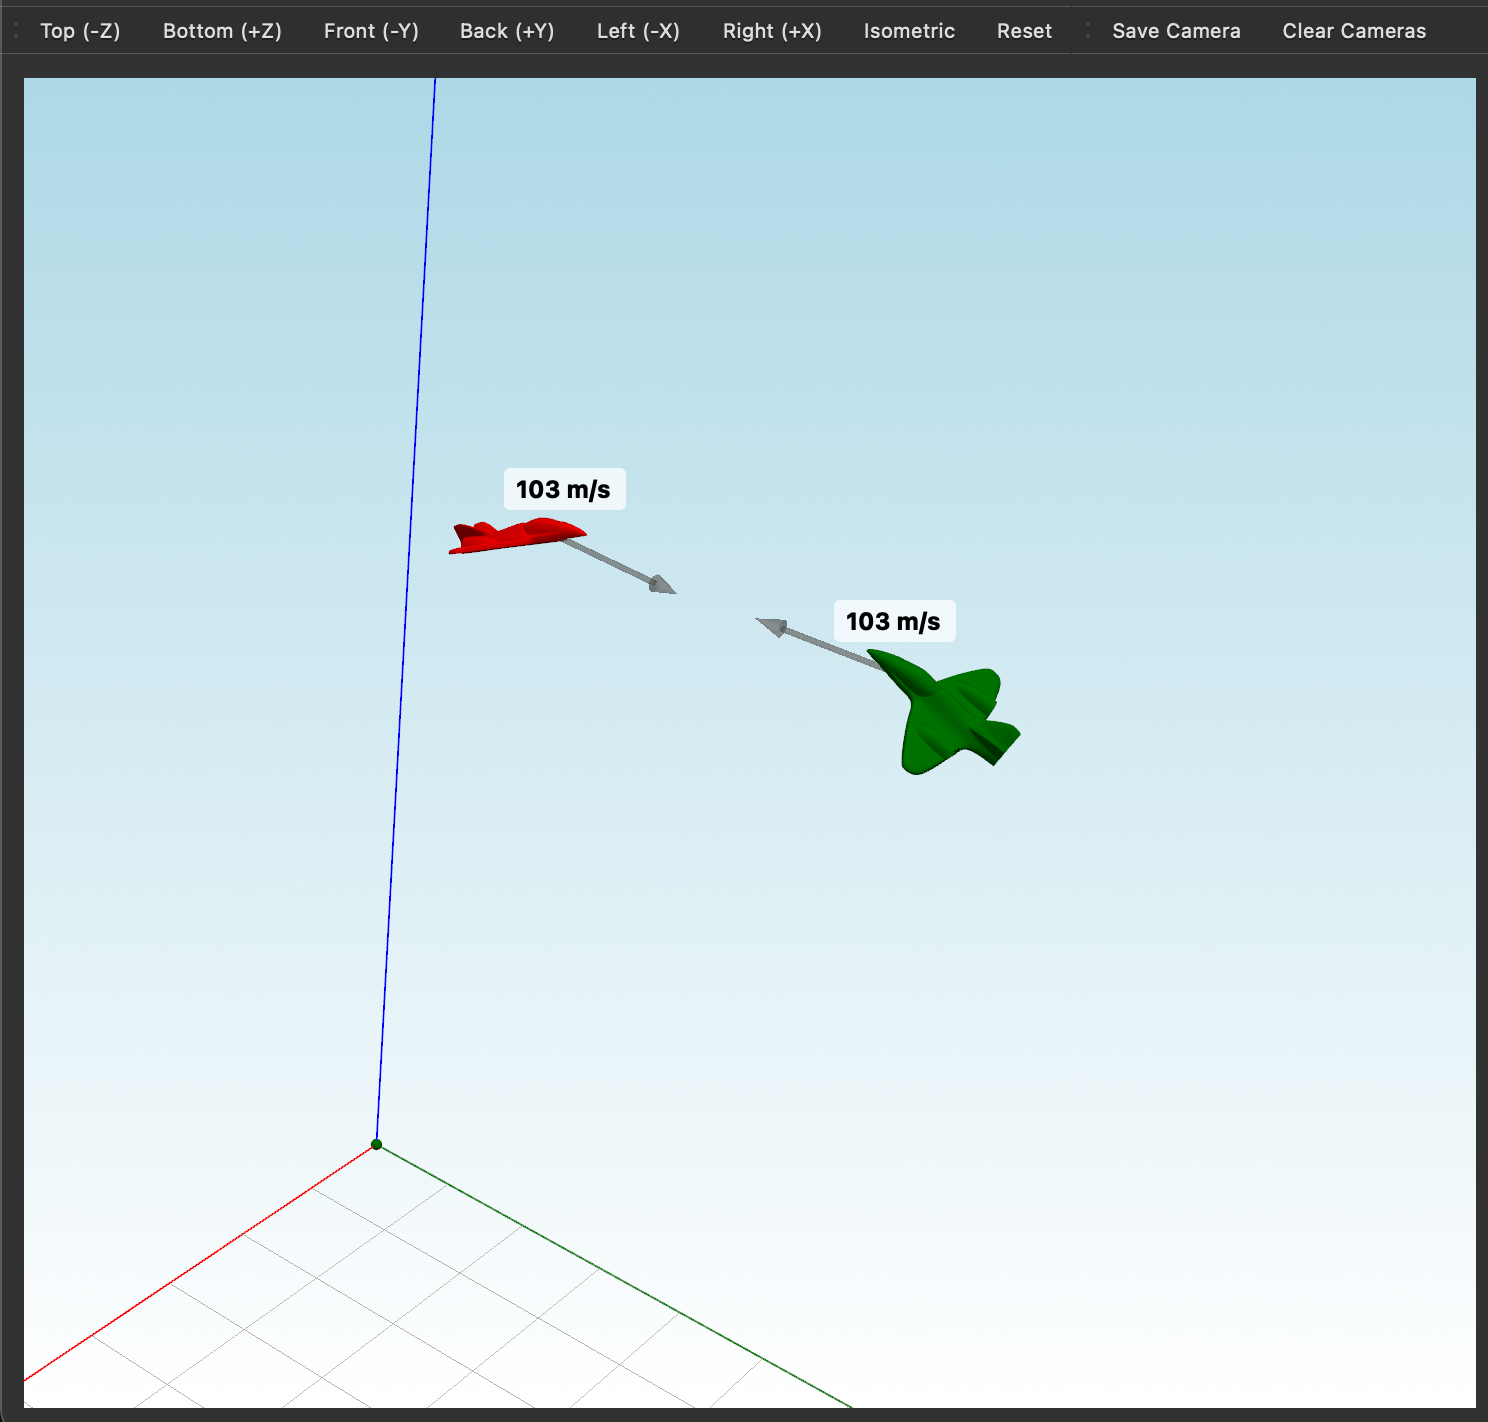
\includegraphics[width=\textwidth]{figures/visualisation/3d_visual.png}
\caption{3D Simulation Visualisation (with additional velocity details)}
\label{fig:3d_visuals}
\end{figure}

\section{Extensions}
\label{sec:3.5}

\subsection{Numba Compilation}
\label{sec:3.5.1}

Numba's JIT compilation was investigated as a performance optimisation for the kinematic calculations in \cref{sec:3.2.3}. This compilation happens on the first call to the function, and subsequent calls need not access the Python interpreter at all, often resulting in significant performance gains. Numba is specifically designed for numerical computation and integrates with NumPy arrays well, making it well suited for the vectorised kinematics of this project. It provides two modes: \texttt{@jit} object mode, which attempts to compile Python code but can fall back to slow interpreted object access if necessary, and \texttt{@njit} no-Python mode, which forces full compilation to machine code and raises an error for unsupported constructs.

No-Python mode was my target as it provides the greatest performance gains, but it imposes constraints on what code can be compiled. Python objects, class instances and much of the standard library are not supported - only NumPy arrays and a subset of NumPy operations are allowed. This motivated design shifts away from OOP as previously discussed, but also demonstrated a trade-off between performance and maintainability. In the original \texttt{step()} function scalar-array polymorphism was supported, and it could accept either a single agent's state or an array of $N$ agent states. This was exploited in the MDP's forward projection, where only the ownship's state needed to be projected forwards. With an \texttt{@njit} decorator this functionality was sacrificed, and the MDP was forced to construct or slice single-element arrays for each scalar as demonstrated in \cref{lst:numba_poly}.

\begin{listing}[H]
\begin{minted}{python}
# Kinematic calculation agent for arrays of N agents
# Used in simulation to step all agents forwards at once
@njit
def step_agents(positions, speeds, ...):
    # equations of motions...

# MDP forward projection
# This fails in @njit - scalar doesn't broadcast.
step_agents(positions[i], speeds[i], ...)

# Fix - explicit single-element slice maintains dimensionality
step_agents(positions[i:i+1], speeds[i:i+1], ...)
\end{minted}
\caption{Scalar-array polymorphism trade-off for \texttt{@njit} broadcasting consistency.}
\label{lst:numba_poly}
\end{listing}

The performance impacts of Numba integration are investigated in the Evaluation chapter.

\subsection{Multi-Agent Runs}
\label{sec:3.5.2}

\subsection{Alternative Behaviours}
\label{sec:3.5.3}

\review{mark scheme says contribution to the field with genuine impact. should I state that stuff that in this chapter? i originally had some stuff about it in the conclusion.}
